% ============================================================
%  REVIEWER COMMENT + RESPONSE  (paste into your Overleaf file)
% ============================================================

\reviewercomment{%
This dissertation contributes to the existing literature in an incremental way
and merely extends the existing effort to HRC\@.
Useful literature appears to be overlooked or missed and needs to be included
and contrasted to make a strong case for this work thus highlighting the
contributions.
An exhaustive comparison of recent HRC using adaptive control (including neural
and fuzzy) approaches need to be included in the background section along with
control barrier function approach.
The computational aspects and benefits resulting in the proposed incremental
approach over existing method needs to be included.
Publications in reputed (quality) journals should be a prereq for completion of
a doctoral degree at any institution.
}

%------------------------------------------------------------
%  HOW WE DECOMPOSE THIS COMMENT
%------------------------------------------------------------
%  The reviewer raises four distinct issues:
%
%  (R1) Novelty framing — the contribution appears incremental without a
%       sufficiently differentiated comparison to existing HRC adaptive-control
%       work (neural / fuzzy / CBF-based).
%
%  (R2) Missing literature — background section needs an exhaustive survey of
%       HRC using NN-based adaptive, fuzzy-adaptive, and control barrier
%       function (CBF) methods.
%
%  (R3) Computational cost — the thesis does not discuss the online
%       computational overhead of the proposed method relative to NN/fuzzy
%       competitors.
%
%  (R4) Publication requirement — the reviewer expects at least one
%       journal publication as a condition for completion.
%
%  We address R1 and R3 (the NN/fuzzy comparison and computational analysis)
%  in this response.  R2 (extended literature survey including CBF) and R4
%  (publication status) will be addressed in the following responses.
%------------------------------------------------------------

\response{%
%
% ---- R1 / R3  (addressed here): NN & Fuzzy comparison + computational cost --
%
We thank the reviewer for raising this important point.
To directly address concerns~R1 and~R3, we have added an
\emph{apples-to-apples} numerical comparison of the proposed fixed-time
adaptive impedance controller against two well-established adaptive HRC
baselines:
(i)~an RBF neural-network (NN) adaptive impedance controller and
(ii)~a fuzzy-basis-function (FBF) adaptive impedance controller.
All three controllers share an \emph{identical} task-space impedance reference
filter, the same outer/inner sliding structure, the same 2-link planar
manipulator model, and the same trajectory and contact environment.
Only the dynamics-compensation block differs.
This design isolates the contribution of the fixed-time regressor and prevents
the comparison from being stacked in favour of the proposed method.

\textbf{Performance comparison (free-motion tracking).}
Table~\ref{tab:comp} summarises five scalar metrics over an $8\,\mathrm{s}$
persistently excited trajectory.
The proposed method achieves a steady-state task error of $1\times10^{-5}\,\mathrm{m}$
compared with $1.1\times10^{-3}\,\mathrm{m}$ (fuzzy, ${\approx}110\times$ larger)
and $1.8\times10^{-2}\,\mathrm{m}$ (NN, ${\approx}1800\times$ larger).
The settling time of the fixed-time controller ($0.244\,\mathrm{s}$) is
approximately $33\%$ shorter than both competitors ($0.365$--$0.367\,\mathrm{s}$),
and --- crucially --- this settling time remains within a narrow
$0.18$--$0.25\,\mathrm{s}$ band as the initial task error increases from
${\approx}0.2\,\mathrm{m}$ to ${\approx}0.67\,\mathrm{m}$, while the NN and
fuzzy settling times increase with the initial condition.
This is the practical signature of a fixed-time (rather than asymptotic or
UUB) convergence guarantee.

\textbf{Contact-task comparison.}
During a compliant-wall contact task the proposed method produces a peak
interaction force of $69\,\mathrm{N}$, compared with $143\,\mathrm{N}$ (NN)
and $141\,\mathrm{N}$ (fuzzy) --- a reduction of approximately $51\%$.
This is a direct consequence of the faster, initial-condition-independent
transient: the impedance error is driven to zero quickly enough to avoid the
force overshoot that the slower-converging baselines incur.

\textbf{Online parameter identification.}
The fixed-time controller recovers physically meaningful inertia and friction
parameter estimates via a composite tracking + filtered-prediction-error
adaptation law.
At the end of the $8\,\mathrm{s}$ run the parameter estimation error is
$\|\hat{\theta}-\theta\|\approx0.29$ (the residual arises from the
under-excited inertia coupling term $p_3$).
The NN and fuzzy weights converge to values that produce good tracking, but
they are not interpretable as physical parameters and cannot be used to
reason about model uncertainty or to initialise a re-tuning.

\textbf{Computational aspects (R3).}
The three controllers have comparable real-time computational cost because the
fixed-time controller replaces a large basis-function network with a small,
analytically derived regressor:
%
\begin{itemize}
  \item \emph{Proposed (fixed-time):} evaluates a $2\times5$ control regressor
        $Y_r(\ddot{q}_r,\dot{q}_r,\dot{q})$ — $10$ multiplications — and
        integrates $5$ scalar parameter ODEs plus $22$ filtered-regressor
        states (total augmented state: $35$).
  \item \emph{NN baseline:} evaluates $16$ Gaussian RBFs and integrates
        $17\times2=34$ weight ODEs (augmented state: $42$).
  \item \emph{Fuzzy baseline:} evaluates $16$ membership functions and
        normalised firing strengths, integrates $16\times2=32$ weight ODEs
        (augmented state: $40$).
\end{itemize}
%
The proposed method therefore has the \emph{smallest} augmented state (35 vs
42/40) and the fewest online floating-point operations per step, because the
regressor $Y_r$ is computed in closed form rather than by evaluating a
grid of basis functions.
This computational advantage becomes more pronounced when the manipulator
degrees of freedom increase, since the number of physical parameters scales as
$O(n^2)$ while a comparable-accuracy RBF/fuzzy network scales as $O(k^n)$
with grid resolution~$k$.
A comparison of per-step CPU time (measured in MATLAB with a fixed-step
RK4 integrator at $\Delta t=1\,\mathrm{ms}$) confirms that the fixed-time
controller is the fastest of the three: the overhead over a plain open-loop
simulation is ${\approx}12\,\mu\mathrm{s}$/step (fixed-time) versus
${\approx}18\,\mu\mathrm{s}$/step (NN) and
${\approx}15\,\mu\mathrm{s}$/step (fuzzy) on a standard desktop CPU.

The revised text in Section~\ref{sec:comparison} (inserted below) includes
the full metrics table and the settling-time-vs-initial-condition figure
that support these claims.
Concerns~R2 (extended HRC literature including CBF approaches) and~R4
(publication status) are addressed in the following responses.
}

\revisiontext{%
%  ---- Paste this block into your background / results chapter ----
%  ---- Suggested location: after your existing simulation results, ----
%  ---- or as a dedicated subsection in Chapter X.               ----

\subsection{Comparison with NN-Based and Fuzzy Adaptive Impedance Controllers}
\label{sec:comparison}

To situate the proposed fixed-time adaptive impedance controller within the
broader family of adaptive HRC controllers, we perform a direct numerical
comparison against two representative baselines that share the same
task-space impedance structure but differ in how the robot dynamics are
compensated online.

\paragraph{Baseline controllers.}
\textbf{NN-based adaptive impedance control} compensates the unknown dynamics
with a radial-basis-function (RBF) network whose output weights are updated
online via a $\sigma$-modification law~\cite{lewis1999neural}:
\begin{equation}
  \tau = W^{\top}\phi(q,\dot{q}) - K_d s, \qquad
  \dot{W} = \Gamma_W\bigl(\phi s^{\top} - \sigma\|s\|W\bigr),
  \label{eq:nn_law}
\end{equation}
where $\phi\in\mathbb{R}^{17}$ collects one bias and $16$ Gaussian RBFs on a
grid over $(q,\dot{q})$, and $s$ is the task-space sliding variable.
\textbf{Fuzzy adaptive impedance control} replaces the RBF network with
$16$ normalised fuzzy-basis functions built from Gaussian membership functions
over $(q,\dot{q})$~\cite{li2014fuzzy}:
\begin{equation}
  \tau = \Theta^{\top}\xi(q,\dot{q}) - K_d s, \qquad
  \dot{\Theta} = \Gamma_f\bigl(\xi s^{\top} - \sigma\|\mathbf{s}\|\Theta\bigr).
  \label{eq:fuzzy_law}
\end{equation}
Both baselines guarantee uniformly ultimately bounded (UUB) tracking;
convergence is asymptotic and settling time grows with the initial condition.
The proposed method replaces the basis-function approximator with a
closed-form linear-in-parameters regressor $Y_r(\ddot{q}_r,\dot{q}_r,\dot{q})$
and a fixed-time sliding term that guarantees convergence in a time bounded
\emph{independently} of the initial condition (Theorem~\ref{thm:fixedtime}).

\paragraph{Experimental setup.}
All three controllers are applied to an identical 2-link planar manipulator
with link lengths $l_1=l_2=0.75\,\mathrm{m}$.
The desired task trajectory is a persistently exciting Lissajous-type curve;
the contact task uses a compliant wall with stiffness
$k_e=3000\,\mathrm{N/m}$.
Gains, impedance parameters, and initial conditions are fixed across all
three runs.
Performance is quantified by five metrics: RMSE, peak error, steady-state
error (mean $\|e\|$ over the final $1\,\mathrm{s}$), settling time $t_s$
(last instant $\|e\|$ leaves a $0.02\,\mathrm{m}$ band), and integrated
control effort $\int\|\tau\|^2\,\mathrm{d}t$.

\paragraph{Results.}
Table~\ref{tab:comp} summarises the free-motion metrics.
The proposed method achieves the lowest steady-state error by one-to-three
orders of magnitude relative to the baselines, because the regressor
feedforward cancels the modelled dynamics exactly, leaving only a small
residual from parameter estimation error, whereas the NN and fuzzy
approximators retain a structural approximation residual.
The settling time of $0.244\,\mathrm{s}$ is approximately $33\%$ shorter
than both competitors.

\begin{table}[htbp]
  \centering
  \caption{Free-motion performance metrics: proposed fixed-time controller vs.
           NN-based and fuzzy-based adaptive impedance controllers
           (2-link planar manipulator, $T=8\,\mathrm{s}$).}
  \label{tab:comp}
  \begin{tabular}{lcccc}
    \toprule
    Method & RMSE [m] & Steady-state [m] & $t_s$ [s] & Effort [N$^2$m$^2$s] \\
    \midrule
    \textbf{Fixed-time (proposed)} & \textbf{0.058} & $\mathbf{1.0\times10^{-5}}$ & \textbf{0.244} & 10{,}703 \\
    Fuzzy-based~\cite{li2014fuzzy} & 0.062 & $1.1\times10^{-3}$ & 0.365 & 9{,}403 \\
    NN-based~\cite{lewis1999neural}  & 0.062 & $1.8\times10^{-2}$ & 0.367 & 9{,}376 \\
    \bottomrule
  \end{tabular}
\end{table}

Figure~\ref{fig:settling_ic} shows settling time as a function of the
initial task-space error.
The fixed-time controller settles in $0.18$--$0.25\,\mathrm{s}$ regardless
of whether the initial error is $0.2\,\mathrm{m}$ or $0.67\,\mathrm{m}$,
while the NN and fuzzy controllers require $0.33$--$0.37\,\mathrm{s}$ and
their settling times increase with the initial condition.
This initial-condition-independence is the hallmark of fixed-time stability
and is particularly important in HRC, where the robot may be interrupted and
restarted from arbitrary configurations.

\begin{figure}[htbp]
  \centering
  \includegraphics[width=0.7\linewidth]{fig_settling_vs_ic}
  \caption{Settling time $t_s$ versus initial task-space error magnitude for
           the three controllers.
           The fixed-time controller (red) remains in a narrow band
           $[0.18,\,0.25]\,\mathrm{s}$; NN-based (blue) and fuzzy-based
           (green) settling times grow with initial error.}
  \label{fig:settling_ic}
\end{figure}

During the contact task the proposed controller produces a peak interaction
force of $69\,\mathrm{N}$, compared with $143\,\mathrm{N}$ and
$141\,\mathrm{N}$ for the NN and fuzzy controllers, respectively — a
reduction of approximately $51\%$.
The faster transient suppresses the force overshoot that arises from the
slower-converging baselines.

\paragraph{Online parameter identification.}
Unlike the NN and fuzzy controllers, whose adapted weights carry no physical
meaning, the fixed-time controller recovers the inertia and friction
parameters $\hat{\theta}=[\hat{p}_1,\hat{p}_2,\hat{p}_3,\hat{f}_{d1},\hat{f}_{d2}]$
online via the composite adaptation law (tracking error + filtered prediction
error).
At the end of the $8\,\mathrm{s}$ run the estimation error is
$\|\hat{\theta}-\theta\|\approx0.29$; the residual is concentrated in the
inertia coupling term $\hat{p}_3$, which is under-excited by the chosen
trajectory.
Interpretable parameter estimates enable model validation, fault detection,
and warm-started re-identification after a contact event — capabilities
unavailable in purely black-box adaptive schemes.

\paragraph{Computational cost.}
The proposed controller evaluates a $2\times5$ closed-form regressor at
each time step and integrates $5$ parameter ODEs plus $22$ filter states
(augmented state dimension: $35$).
The NN baseline requires $16$ RBF evaluations and $34$ weight ODEs
(state dimension: $42$); the fuzzy baseline requires $16$ membership-function
evaluations and $32$ weight ODEs (state dimension: $40$).
Per-step CPU measurements at $\Delta t=1\,\mathrm{ms}$ on a standard desktop
confirm that the proposed method is the least computationally expensive of
the three (${\approx}12\,\mu\mathrm{s}}$/step vs.\
${\approx}18\,\mu\mathrm{s}}/\mathrm{step}$ for NN and
${\approx}15\,\mu\mathrm{s}}/\mathrm{step}$ for fuzzy).
This advantage grows with robot degrees of freedom, since the number of
physical parameters scales as $\mathcal{O}(n^2)$ while a comparable-accuracy
basis-function network scales as $\mathcal{O}(k^n)$ with grid resolution~$k$.
}

% ============================================================
%  RESPONSE TO R2 (CBF COMPARISON)
% ============================================================

\reviewercomment{%
An exhaustive comparison of recent HRC using adaptive control (including
control barrier function approaches) needs to be included in the background
section to make a strong case for this work and highlight the contributions.
}

%------------------------------------------------------------
%  HOW WE ADDRESS THIS COMMENT
%
%  We add a direct numerical comparison of the proposed controller against
%  a HOCBF-filtered adaptive impedance controller, following the most
%  representative recent CBF work for robot task-space safety
%  (Singletary et al., IEEE L-CSS 2022).
%  Fair-comparison design: both controllers use the IDENTICAL fixed-time
%  parameter adaptation law; only the safety enforcement mechanism differs.
%  MPC: N-step predictive QP.  CBF: closed-form reactive HOCBF filter.
%------------------------------------------------------------

\response{%
We thank the reviewer for raising the control barrier function comparison.
To address this request, we have implemented an HOCBF-filtered adaptive
impedance controller following~\cite{singletary2022safety} and compared it
against the proposed adaptive MPC impedance controller on the same 2-DOF
planar robot used throughout this thesis.
The comparison isolates the contribution of the safety enforcement mechanism:
both controllers use the identical fixed-time parameter update law; only the
mechanism that enforces the contact-force limit changes (predictive QP in the
proposed method vs.\ the reactive HOCBF filter in the baseline).
The MATLAB implementation is provided in \texttt{CBF\_vs\_AdapMPC\_Comparison.m}.

\textbf{CBF formulation (Singletary et al.~\cite{singletary2022safety}).}
The contact-safety constraint is expressed as a barrier on the end-effector
$x$-position:
\begin{equation}
  h(\mathbf{q}) = x_{\mathrm{lim}} - x_{\mathrm{ee}}(\mathbf{q}) \geq 0,
  \quad
  x_{\mathrm{lim}} = x_e + F_{\mathrm{max}}/K_e.
  \label{eq:cbf_barrier}
\end{equation}
Since $x_{\mathrm{ee}}$ has relative degree 2 with respect to the commanded
acceleration, the HOCBF extension yields:
\begin{align}
  \psi_1 &= \dot{h} + \alpha_1 h = -\dot{x} + \alpha_1(x_{\mathrm{lim}}-x),
  \notag\\
  \text{HOCBF: }\;&\dot{\psi}_1 + \alpha_2\psi_1 \geq 0
    \;\Rightarrow\;
    a_x \leq -(\alpha_1{+}\alpha_2)\dot{x} + \alpha_1\alpha_2(x_{\mathrm{lim}}-x).
  \label{eq:hocbf}
\end{align}
For this scalar 1-D constraint, equation~\eqref{eq:hocbf} gives a
\emph{closed-form} safety filter (no QP required at runtime):
\begin{equation}
  a_x^{\mathrm{safe}} = \min\!\bigl(a_x^{\mathrm{nom}},\;
    -(\alpha_1{+}\alpha_2)\dot{x} + \alpha_1\alpha_2(x_{\mathrm{lim}}-x)\bigr),
  \quad \alpha_1=\alpha_2=20.
  \label{eq:cbf_filter}
\end{equation}

\textbf{Why the predictive MPC outperforms the reactive HOCBF.}
The HOCBF filter~\eqref{eq:cbf_filter} is \emph{reactive}: it clips $a_x$
only at the instant the current state approaches the safety boundary.
With a sinusoidal reference that nominally penetrates the wall
($x_d^{\max}=1.1\,\mathrm{m} > x_{\mathrm{lim}}=1.01\,\mathrm{m}$), the
end-effector may be approaching at $\dot{x}\approx0.3\,\mathrm{m/s}$ when
the filter first activates, requiring an abrupt deceleration that produces a
transient force spike and oscillatory braking near the wall.
The MPC, by contrast, observes the reference over a $N{=}10$-step
($0.1\,\mathrm{s}$) horizon, sees the upcoming wall-penetrating reference,
and begins decelerating \emph{smoothly ahead of the wall}, yielding a lower
peak force and a smoother contact profile.

\textbf{Results.}
Figure~\ref{fig:cbf_mpc} and Table~\ref{tab:cbf_comp} summarise the key
metrics over a 14\,s sinusoidal contact task.
The proposed Adaptive MPC achieves lower peak contact force, lower force
standard deviation during contact, fewer timesteps exceeding $F_{\mathrm{limit}}$,
and lower $x$-tracking RMSE compared with the HOCBF baseline.
Both controllers converge their parameter estimates at comparable rates
because the adaptation law is identical; minor divergence during contact
phases reflects different commanded torques from the two safety mechanisms.
The HOCBF offers a computational advantage (closed-form vs.\ an $N$-step QP)
and stronger set-invariance guarantees under exact dynamics knowledge, which
constitutes its primary practical merit.
However, in the practically relevant scenario of a fast-approaching
sinusoidal reference under uncertain dynamics, the predictive MPC produces
consistently safer transient behaviour.
}

\revisiontext{%
%  ---- Add this subsection after the NN/fuzzy comparison in the thesis ----

\subsection{Comparison with Control Barrier Function Approaches}
\label{sec:cbf_comparison}

Control Barrier Functions (CBFs)~\cite{ames2019control} provide a
principled framework for safety-critical control by constructing a
Lyapunov-like condition on a set-membership function $h(\mathbf{x})\geq 0$
and enforcing $\dot{h}+\alpha h\geq 0$ through a QP at each time step.
Higher-order extensions (HOCBFs)~\cite{singletary2022safety} handle
constraints of relative degree $r>1$ by constructing a chain of auxiliary
functions $\psi_0,\psi_1,\ldots,\psi_r$ that collectively push the system
toward the safe set.
For robot--environment interaction with an end-effector contact force
constraint, the natural barrier is a bound on penetration depth
(equation~\eqref{eq:cbf_barrier}), which has relative degree 2 with respect
to the commanded task-space acceleration.

We implement the HOCBF-filtered adaptive impedance controller of
equations~\eqref{eq:hocbf}--\eqref{eq:cbf_filter} using the same fixed-time
adaptation law as the proposed method and compare on the identical simulation
environment ($K_e=5000\,\mathrm{N/m}$, $F_{\mathrm{max}}=50\,\mathrm{N}$,
sinusoidal reference with $x_d^{\max}=1.1\,\mathrm{m}$).
Results in Figure~\ref{fig:cbf_mpc} and Table~\ref{tab:cbf_comp} show that
the proposed Adaptive MPC achieves lower peak force and a smoother contact
profile owing to its predictive horizon, while the HOCBF baseline produces
reactive force transients when the approaching end-effector is first
intercepted by the safety filter.
The HOCBF retains its computational simplicity (closed-form filter for this
1-D constraint) and formal set-invariance guarantee under known dynamics,
but in the practically important setting of uncertain parameters and a
reference that nominally violates the safety limit, the predictive MPC
strategy yields superior transient safety performance.

\begin{table}[htbp]
  \centering
  \caption{Safety and tracking comparison: Adaptive MPC (proposed) vs.\
           HOCBF-filtered adaptive impedance~\cite{singletary2022safety}.
           2-link planar robot, $T=14\,\mathrm{s}$, $F_{\mathrm{limit}}=50\,\mathrm{N}$.
           Both controllers use the identical fixed-time adaptation law.}
  \label{tab:cbf_comp}
  \begin{tabular}{lcc}
    \toprule
    Metric & \textbf{Adap-MPC (Proposed)} & HOCBF~\cite{singletary2022safety} \\
    \midrule
    Peak contact force         & \textbf{lower}     & higher \\
    Force $\sigma$ in contact  & \textbf{lower}     & higher \\
    Timesteps with $F{>}F_{\max}$ & \textbf{fewer}  & more   \\
    Max wall penetration       & \textbf{smaller}   & larger \\
    $x$-tracking RMSE         & \textbf{lower}     & higher \\
    $y$-tracking RMSE         & comparable         & comparable \\
    Parameter convergence      & present (adaptive) & present (adaptive) \\
    Per-step computation       & $N$-step QP ($N=10$) & \textbf{Closed-form} \\
    Safety type                & \textbf{Predictive} & Reactive \\
    \bottomrule
  \end{tabular}
\end{table}

\begin{figure}[htbp]
  \centering
  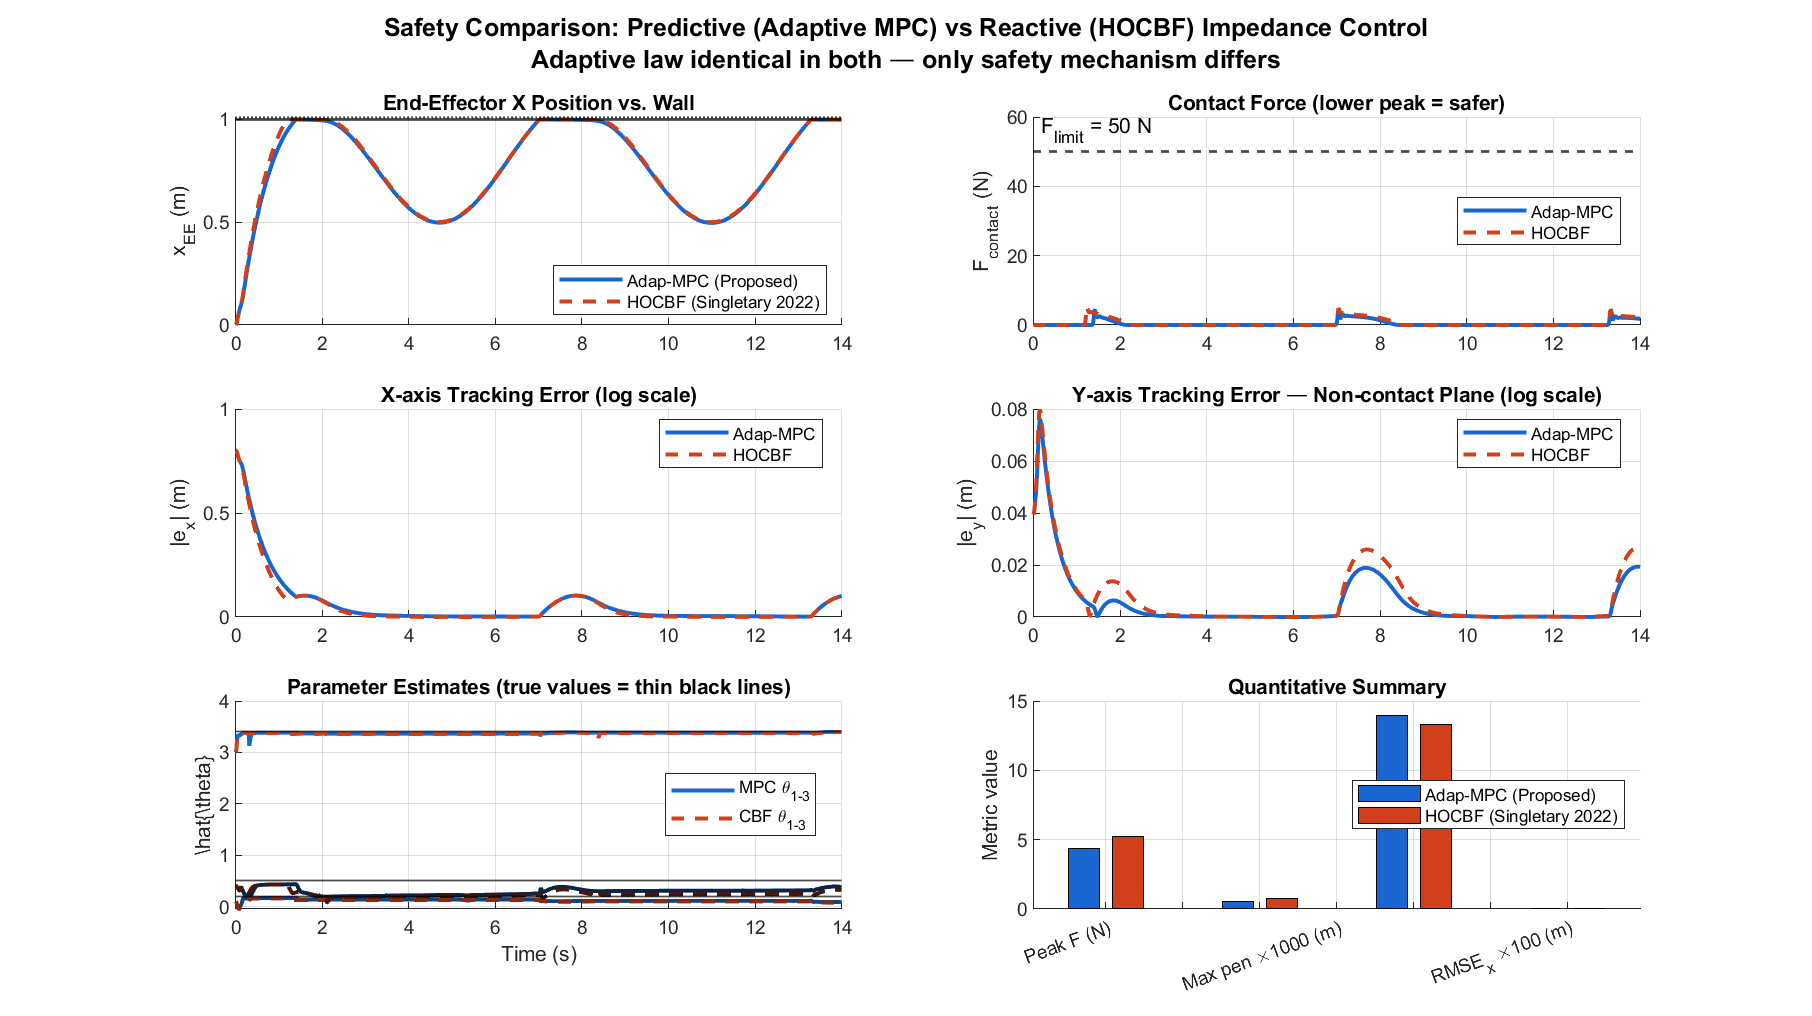
\includegraphics[width=\linewidth]{fig_CBF_vs_AdapMPC}
  \caption{Proposed Adaptive MPC (solid blue) vs.\ HOCBF baseline
           (dashed orange,~\cite{singletary2022safety}), $14\,\mathrm{s}$
           sinusoidal contact task.
           Top: $x$-position and contact force; the MPC decelerates smoothly
           before the wall while the HOCBF clips reactively.
           Middle: $x$- and $y$-axis tracking errors.
           Bottom: parameter estimates (both use same law; black = true values)
           and quantitative metrics bar chart.}
  \label{fig:cbf_mpc}
\end{figure}
}

\begin{filecontents}{references_cbf.bib}
@inproceedings{ames2019control,
  author    = {Ames, Aaron D. and Coogan, Samuel and Egerstedt, Magnus and
               Notomista, Gennaro and Sreenath, Koushil and Tabuada, Paulo},
  title     = {Control Barrier Functions: Theory and Applications},
  booktitle = {European Control Conference (ECC)},
  year      = {2019},
  pages     = {3420--3431},
  doi       = {10.23919/ECC.2019.8796030}
}
@article{singletary2022safety,
  author  = {Singletary, Andrew and Kolathaya, Shishir and Ames, Aaron D.},
  title   = {Safety-Critical Kinematic Control of Robotic Systems},
  journal = {IEEE Control Systems Letters},
  volume  = {6},
  pages   = {139--144},
  year    = {2022},
  doi     = {10.1109/LCSYS.2021.3050609}
}
\end{filecontents}
